\section{Heatwave Application}

\begin{frame}{Motivation}

  \begin{columns}
    \begin{column}{0.6\linewidth}
      \begin{itemize}
        \item Measuring the effect of climate disasters
            \begin{itemize}
            \item Experimental approaches - if not unethical - are nearly impossible
            \item Researchers are stuck with observational data
            \item Recovering robust causal effects is critical policy input
            \end{itemize}
      \end{itemize}
    \end{column}
    \begin{column}{0.4\linewidth}
      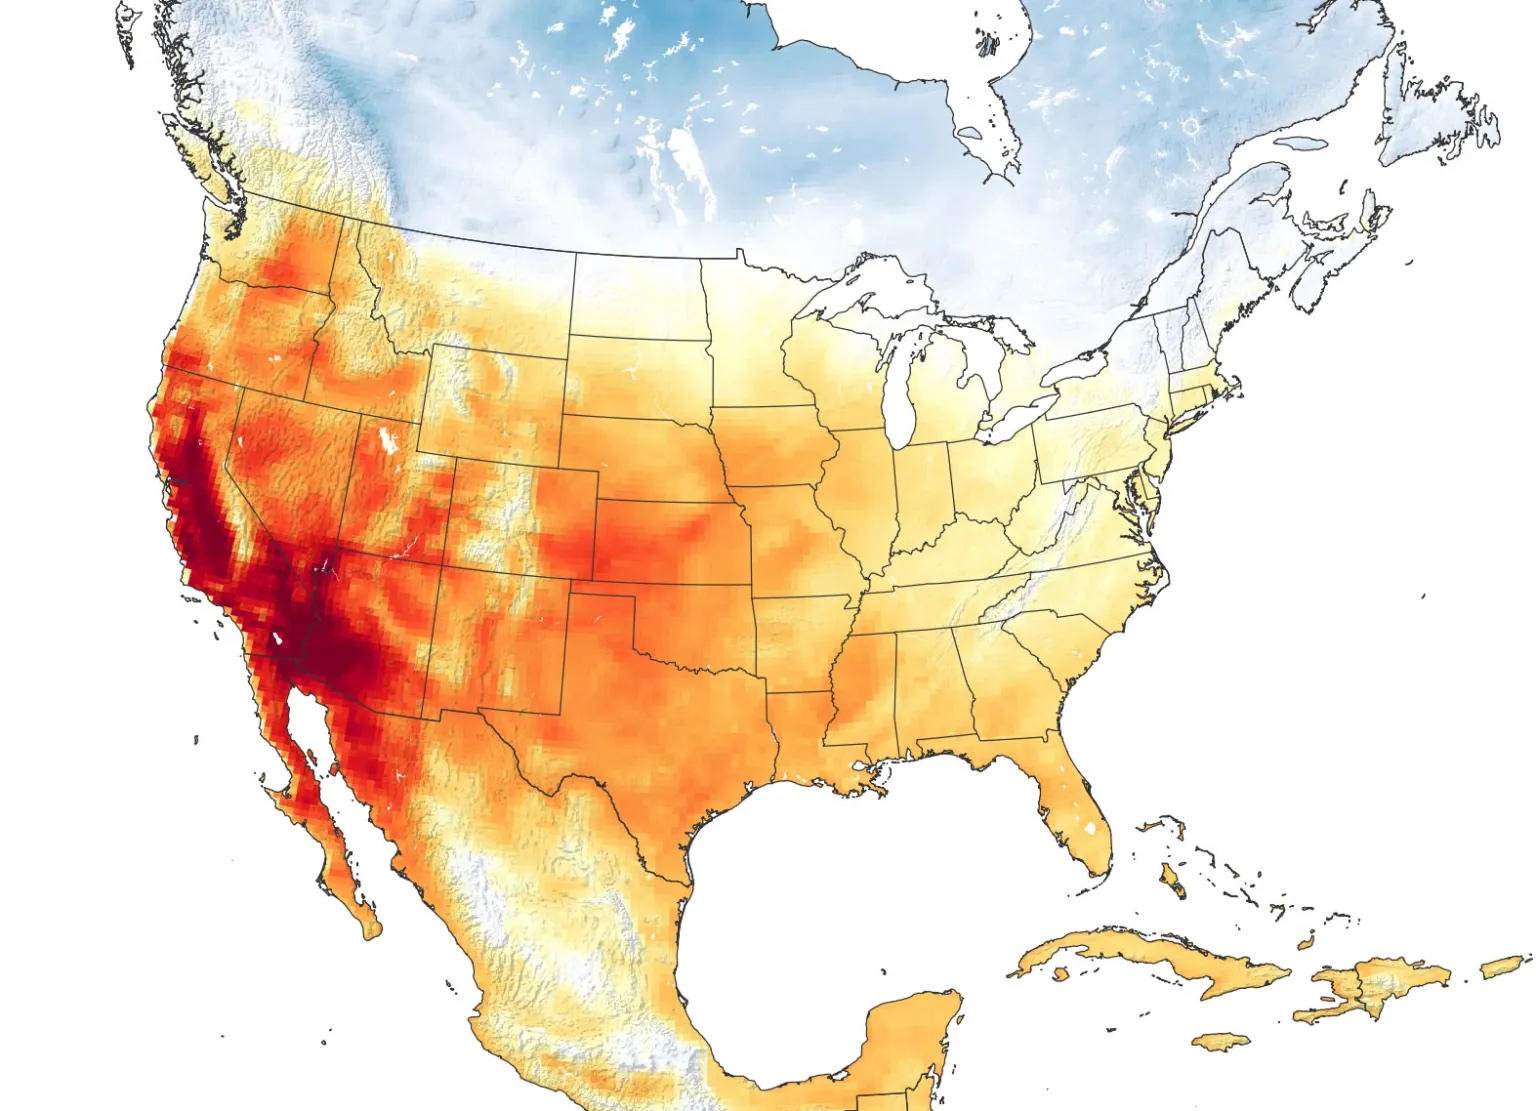
\includegraphics[scale=0.1]{figures/california-heatwave-2020-nasa-eo.jpeg}
      \caption{}
    \end{column}
  \end{columns}

\vspace{7pt}
\begin{center}
    Application: How do we measure the effect of heat waves on community health?
\end{center}

  \note{
    This slide has notes too.
  }

\end{frame}

\begin{frame}{Colorado Cell Phone Ping Data}
- E&E Lab cell phone ping data
- Data Use: Assign unit treated if it moved to hospital
\end{frame}